\section{Manifold}

\begin{frame}
	\begin{block}{Artigo 02}
	\begin{enumerate}
		\item Manifold: A Model-Agnostic Framework for Interpretation and Diagnosis of Machine Learning Models \cite{Manifold}
	\end{enumerate}
	\end{block}
\end{frame}


\begin{frame}
	\begin{block}{Manifold - overview}
		\begin{enumerate}
			\item É um framework para ajudar o cientista a localizar falhas no modelo, para tal, os autores automatizam tarefas típicas para depurar modelos.
			\item Para tal, os autores criaram uma ``matriz de confusão'' que relaciona modelos e classes, com essa matriz é possível avaliar visualmente onde os modelos não concordam.
		\end{enumerate}
	\end{block}
\end{frame}


\begin{frame}
	\begin{block}{Manifold - overview}
				\begin{figure}[!htb]
			\centering	  				
			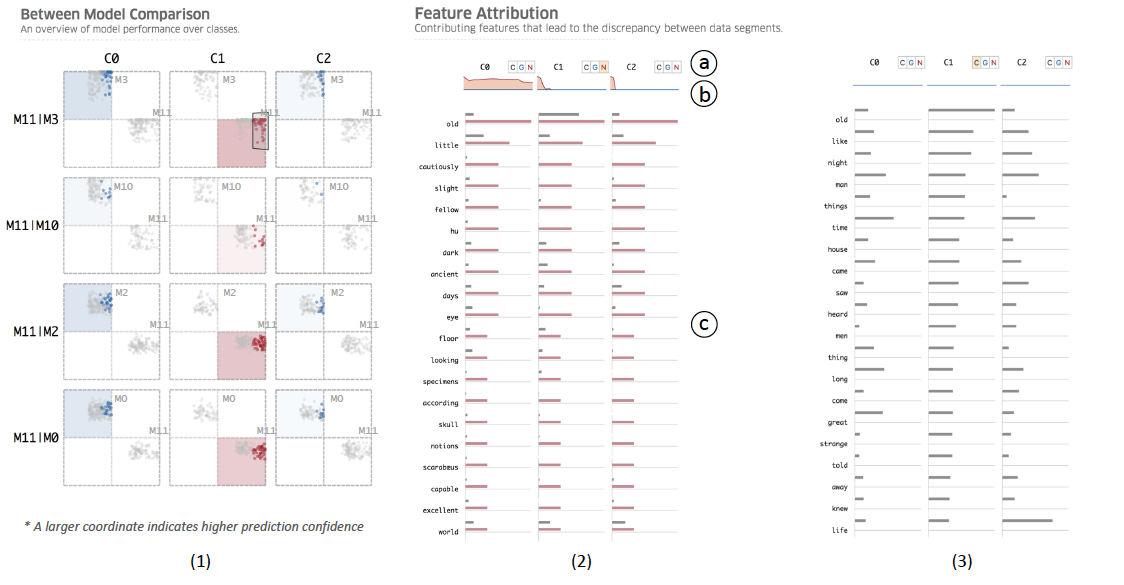
\includegraphics[height=4cm, width = 10cm]{./pic/manifold.png}
			\caption{Visualização sugerida pelo manifold \cite{Manifold}}
			\label{fig_ds_process}
		\end{figure}	
	\end{block}
\end{frame}


\begin{frame}
	\begin{block}{Manifold - overview}
		\begin{enumerate}
			\item Após selecionar a célula (tipicamente será escolhida a células de diferença Q1, Q3) é exibida uma comparação da distribuição de variáveis das instâncias daquela célula.
			\item No próximo gráfico é exibida uma sumarização dos valores (TF-IDF) das features, das instâncias selecionadas, e das instâncias pertencentes a cada classe.
			\item Pode-se usar o gráfico do meio para avaliar quais features são mais relevantes para classificar uma instância em determinada classe
		\end{enumerate}
	\end{block}
\end{frame}


\begin{frame}
	\begin{block}{Manifold - funcionamento}
		\begin{enumerate}
			\item A comparação de modelos é feita por meio de visualização das probabilidades e classes verdadeiras em uma ``matriz de confusão''
		\end{enumerate}
		\begin{figure}[!htb]
			\centering	  				
			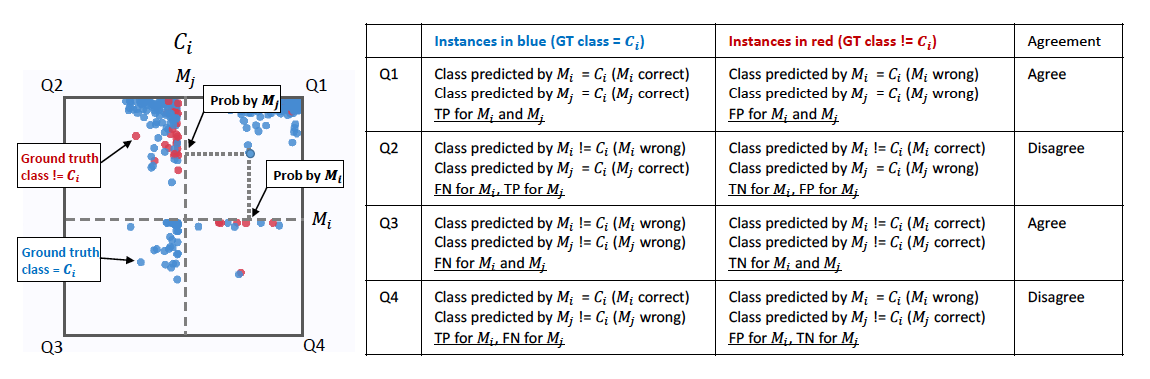
\includegraphics[height=4cm, width = 10cm]{./pic/matrizManifold.png}
			\caption{Matriz de confusão usada pelo Manifold \cite{Manifold}}
			\label{fig_ds_process}
		\end{figure}	
	\end{block}
\end{frame}


\begin{frame}
	\begin{block}{Manifold - funcionamento}
		\begin{enumerate}
			\item A avaliação de importância de features (segundo gráfico da esquerda para direita) é realizada usando uma métrica como TF-IDF para a classe e para o conjunto de dados classificados
			\item Os gráficos acima, que não é a distribuição de variáveis mas a \emph{Kullback-Leibler divergence}, indica o quanto a distribuição dos itens selecionados é parecida com a classe em questão
			\item O último gráfico (da esquerda para direita) mostra a distribuição de features por classe, sumarizadas por TD-IDF
		\end{enumerate}
	\end{block}
\end{frame}

